\documentclass[10pt,a4paper]{report}
\usepackage[utf8]{inputenc}
\usepackage[russian]{babel}
\usepackage[OT1]{fontenc}
\usepackage{amsmath}
\usepackage{amsfonts}
\usepackage{amssymb}
\usepackage{graphicx}
\begin{document}
\title{Описание протокола}
\chapter{Задание}
Разработать клиент-сервурную систему сетевого форума из сервера сетевого форума и пользовательских клиентов.
\section{Основные возможности сервера}
\item Прослушивание определенного порта
\item Обработка запросов на подключение по этому порту от клиентов
\item Поддержка работы нескольких клиентов через механизм нитей
\item Регистрация подключившегося клиента
\item Выдача клиенту перечня новых сообщений форума
\item Выдача клиенту иерархического представление форума
\item Прием от клиента сообщения в ветку форума
\item Выдача списка текущих активных пользователей форума
\item Обработка запроса на отключения клиента
\item Принудительное отключение клиента
\section{Основные возможности клиента}
\item Установление соединения с сервером
\item Посылка регистрационных данных клиента
\item Получение и вывод перечня новых сообщений 
\item Получение и вывод иерархии форума
\item Выбор текущей ветки форума
\item Посылка сообщений в текущую ветку форума
\item Разрыв соединения
\item Обработка ситуации отключения клиента сервером
\chapter{Нефункциональные требования}
\section{Требования к реализации}
Соединение начинает сервер, отправляя приглашение к авторизации. Далее клиент пересылает свой логин и пароль. После этого пользователь может просматривать форум (его иерархию и отдельные сообщения), оставлять сообщения в выбранную ветку форума. После завершения работы клиент должен разорвать соединение.
\section{Требования к надежности}
Длинна принимаемого сервером пакета должна быть ограничена, для избежания падения сервера. Так же мы должны обрабатывать неправильные (неккоректные) запросы от клиента.
\chapter{Накладываемые ограничения}
\item Ограничение на длинну пакета (256 символов)
\item "Белый список" команд
\chapter{Описание архитектуры}
\item При запуске сервера выводится сообщение, просящее ввести имя пользователя и пароль. Процедура повторяется пока пользователь не введет корректную пару логин/пароль. Пользователь может завершить сеанс командой exit.
\item При авторизации пользователя на экран выводятся еще не прочитанные им посты
\item При введении команды posts выводится структура форума
\item При введении команды show id_post выводится сообщение форума
\item При введении команды online выводится список активных пользователей
\item При введении команды add пользователю предлагается ввести имя темы, название поста и сообщение поста, после чего сообщение будет добавлено новое сообщение
Ниже представлена sequence - диаграмма работы клиента - сервера
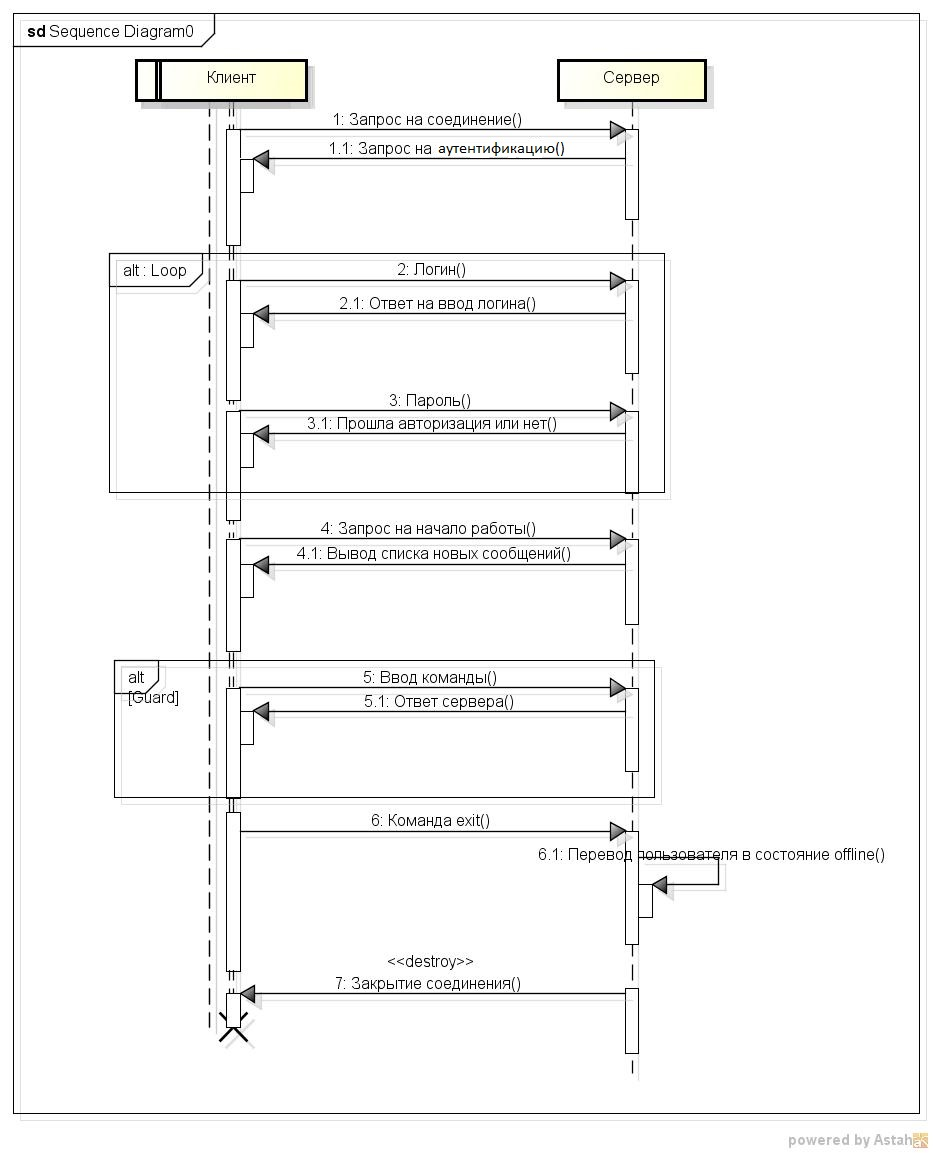
\includegraphics[scale=0.9]{diagram}
\end{document}